\documentclass[a4paper,11pt]{article}

\usepackage[utf8]{inputenc}

\usepackage{graphicx}
\usepackage{caption}
\usepackage{subcaption}

\usepackage{hyperref}

\usepackage{pgfplots}
\pgfplotsset{compat=1.18} 

\usepackage{minted}

\begin{document}

\title{
    \textbf{Assignment 5 Report - Linked List in Java}
}
\author{Dean Tsankov}
\date{\today}

\maketitle

\section*{Introduction}

In this report I will present the concept and implementation of a simple data structure, known as a linked list. Each of its elements (or cells) will hold a value and a reference to another data structure. This turns out to be the simplest linked data structure that can be and yet it will behave quite differently from the array structures that we have been using so far. Along with the linked list implementation itself I will compare how an append function between two lists fairs against a similar append operation between two arrays. And lastly I will explore how this new structure can be used to replace my dynamic array stack implementation from the second assignment.

\section*{The linked list implementation}
As stated previously a linked list consists of multiple elements each of which holds some useful value called here the {\tt head}, and also a reference variable pointing to the next element in the list (here called the {\tt tail}). The last element does not point to any other element and so its tail has a {\tt null} value. Here is how we define a simple cell of the list:

\begin{minted}[
frame=single,
framesep=2mm,
baselinestretch=1.2,
fontsize=\footnotesize,
]{java}
    (...)
    private class Cell {
        int head;
        Cell tail;

        Cell(int val, Cell tl) {
            head = val;
            tail = tl;
        }
    }
    (...)
\end{minted}

Later on the general linked list structure needs to only keep track of pointing to the first element, since afterwords all others point to the following in the list. 
\\

Some of the methods which are useful to have in such a structure are presented bellow:

\begin{minted}[
frame=single,
framesep=2mm,
baselinestretch=1.2,
fontsize=\footnotesize,
]{java}
    (...)
    void add(int item) {
        Cell newCell = new Cell(item, this.first);
        this.first = newCell;
    }
    (...)
\end{minted}

Adding a new element to the list simply creates a cell which points to the current first element of the list and then changes that said first element reference to point to the newly created cell.

\begin{minted}[
frame=single,
framesep=2mm,
baselinestretch=1.2,
fontsize=\footnotesize,
]{java}
    (...)
    int length() {
        int i = 0;
        Cell itr = this.first;
        while (itr != null) {
            i++;
            itr = itr.tail;

        }
        return i;
    }
    (...)
\end{minted}

In order to find the length of the list we have to traverse it and count each iteration. We do this by taking an iteration cell beginning from the first element in the list and going to its tail reference while checking if it is not null as that would mean that we are at the end, so we can return the counter variable.

\begin{minted}[
frame=single,
framesep=2mm,
baselinestretch=1.2,
fontsize=\footnotesize,
]{java}
    (...)
    boolean find(int item) {
        Cell itr = this.first;
        while (itr != null) {
            if (itr.head == item) {
                return true;
            }
            itr = itr.tail;
        }
        return false;
    }
    (...)
\end{minted}

Finding a specific element requires the same sort of iteration through the list. This time, though, we check the head value of each element in order to find a match.

\begin{minted}[
frame=single,
framesep=2mm,
baselinestretch=1.2,
fontsize=\footnotesize,
]{java}
    (...)
    void remove(int item) {
        Cell itr = this.first;
        Cell prev = null;
        while (itr != null) {
            if (itr.head == item) {
                if (prev != null) {
                    prev.tail = itr.tail;
                } else {
                    this.first = itr.tail;
                }
                break;
            }
            prev = itr;
            itr = itr.tail;
        }
    }
    (...)
\end{minted}
Removing an element requires us to not only keep track of the current element we are iteration over but also the previous one, since when we want to remove an element we make the previous element's tail pointer refer to the current one's tail element. Thus we are in essence making the list skip over the element we removed.

\begin{minted}[
frame=single,
framesep=2mm,
baselinestretch=1.2,
fontsize=\footnotesize,
]{java}
    (...)
    public void append(LinkedList b) {
        Cell nxt = this.first;
        Cell prev = null;
        while (nxt.tail != null) {
            prev = nxt;
            nxt = nxt.tail;
        }
        nxt.tail = b.first;
        b.first = null;
    }
    (...)
\end{minted}

Lastly appending is the very simple action of making the last element's tail variable point to the first element of the list we want to append.
\\

For debugging purposes I also overwrote the {\tt ToString} method as such.

\begin{minted}[
frame=single,
framesep=2mm,
baselinestretch=1.2,
fontsize=\footnotesize,
]{java}
    (...)
    public String ToString() {
        Cell nxt = this.first;
        StringBuilder str = new StringBuilder();
        while (nxt != null) {
            str.append(nxt.head).append(' ');
            nxt = nxt.tail;
        }
        return str.toString();
    }
    (...)
\end{minted}

\section*{Bench-marking the append complexity of the linked list}

Now I will set up a benchmark that gives an idea of the run
time of the append operation. Initially the size of the first linked
list (a) will be varied and appended to a fixed size linked list (b). The linked lists are generated with the provided code which basically gives each element the value of its "index". 
\\

If we think about what the append algorithm is doing, it goes trough all elements of the first list and does not particularly need to iterate through the elements of the second one. So when, in this case, the first list's size is varied and the second is constant, we should expect that the runtime complexity would be related to the size of the list (a).
\\

Taking a look at the graphical plot:

\begin{figure}[H]
    \centering
    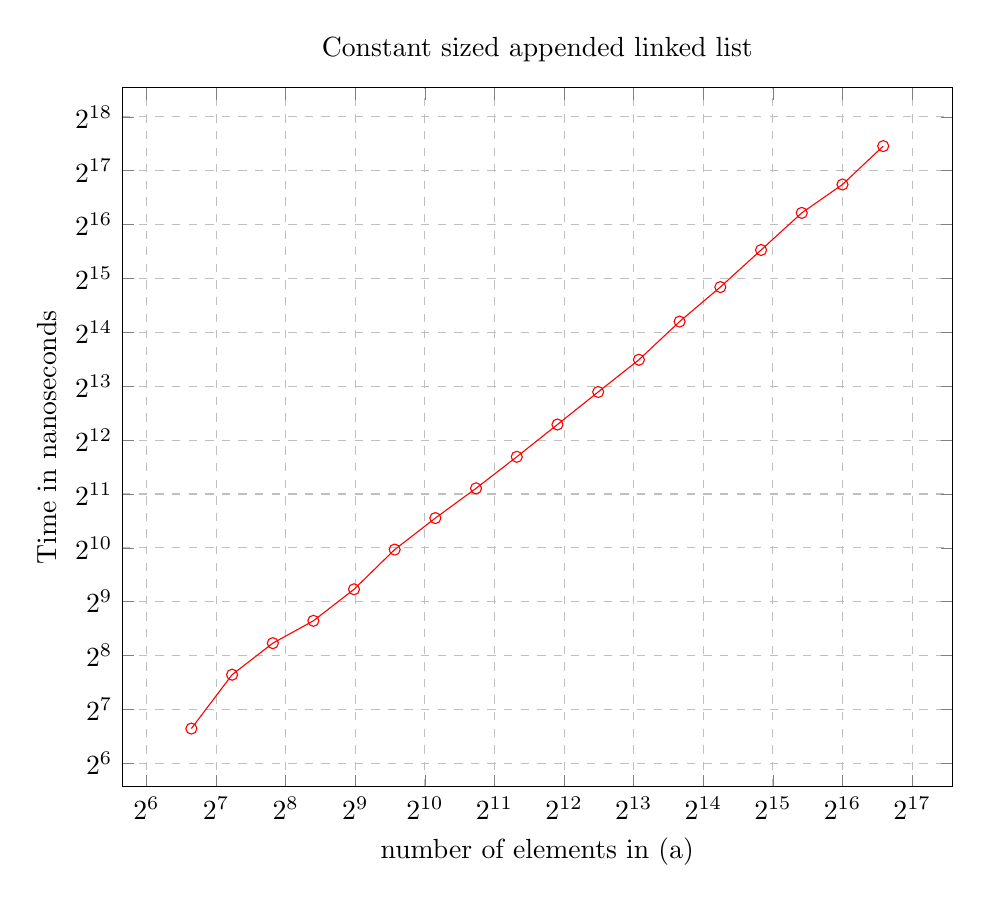
\begin{tikzpicture}
        \begin{axis}[
            title={Constant sized appended linked list},
            width=\linewidth,
            xlabel={number of elements in (a)},
            ylabel={Time in nanoseconds},
            xmode=log,
            log basis x={2},
            ymode=log,
            log basis y={2},
            ymajorgrids=true,
            xmajorgrids=true,
            grid style=dashed,
        ]
        
        \addplot[
            color=red,
            mark=o,
            ]
            coordinates {
            (100,100)(150,200)(225,300)(337,400)(505,600)(757,1000)(1135,1500)(1702,2200)(2553,3300)(3829,5000)(5743,7600)(8614,11500)(12921,18800)(19381,29300)(29071,47200)(43606,76100)(65409,109700)(98113,179700)
            };
            
            
        \end{axis}
        \end{tikzpicture}
    \caption{Linked list append operation benchmark}
    \label{fig:plot1}
\end{figure}

It does in fact follow that this scenario follows a linear complexity represented by {\tt O(n)} with n being the length of the first list (a).
\\

The next case we would be interested in is the one where the first list has a constant length and the second one is changed. As discussed above appending works only by having to traverse the first list and as such we should expect a constant time complexity as we have no variation in its size.

\begin{figure}[H]
    \centering
    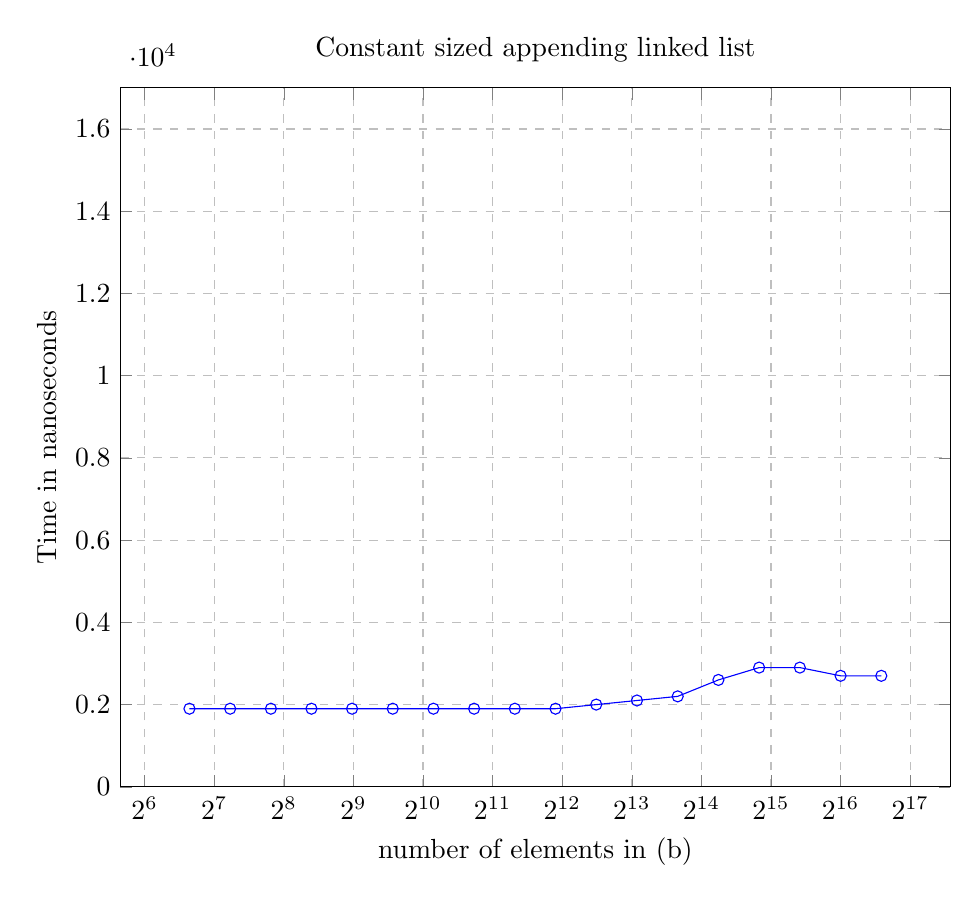
\begin{tikzpicture}
        \begin{axis}[
            title={Constant sized appending linked list},
            width=\linewidth,
            xlabel={number of elements in (b)},
            ylabel={Time in nanoseconds},
            xmode=log,
            log basis x={2},
            ymin=0, ymax=17000,
            ymajorgrids=true,
            xmajorgrids=true,
            grid style=dashed,
        ]
        
        \addplot[
            color=blue,
            mark=o,
            ]
            coordinates {
            (100,1900)(150,1900)(225,1900)(337,1900)(505,1900)(757,1900)(1135,1900)(1702,1900)(2553,1900)(3829,1900)(5743,2000)(8614,2100)(12921,2200)(19381,2600)(29071,2900)(43606,2900)(65409,2700)(98113,2700)
            };
            
            
        \end{axis}
        \end{tikzpicture}
    \caption{Linked list append operation benchmark}
    \label{fig:plot1}
\end{figure}

Evidently for the most part this holds true and the graph is nearing constant complexity, meaning {\tt O(1)}.

\section*{Array comparison}

As the data structure we have been most familiar with, it might be useful to see how arrays compare to linked lists. I will do the same two benchmarks of an append function implemented for arrays.

\begin{minted}[
frame=single,
framesep=2mm,
baselinestretch=1.2,
fontsize=\footnotesize,
]{java}
    (...)
    public static int[] arrayAppend(int[] a, int[] b) {
        int[] result = new int[a.length + b.length];
        for (int i = 0; i < a.length; i++) {
            result[i] = a[i];
        }
        for (int i = 0; i < b.length; i++) {
            result[a.length + i] = b[i];
        }
        return result;
    }
    (...)
\end{minted}

The way this array append works is that it creates a new array with size equal to the sum of the two arrays we want to join together. The new array is filled first with the elements from (a) and then the ones from (b). Here unlike the linked list implementation we are always required to go through both the appending and the appended arrays.

As is we would expect the complexity to be linear. The following graph has a logarithmicaly scaled x-axis so the graph is actually nearing a line.

\begin{figure}[H]
    \centering
    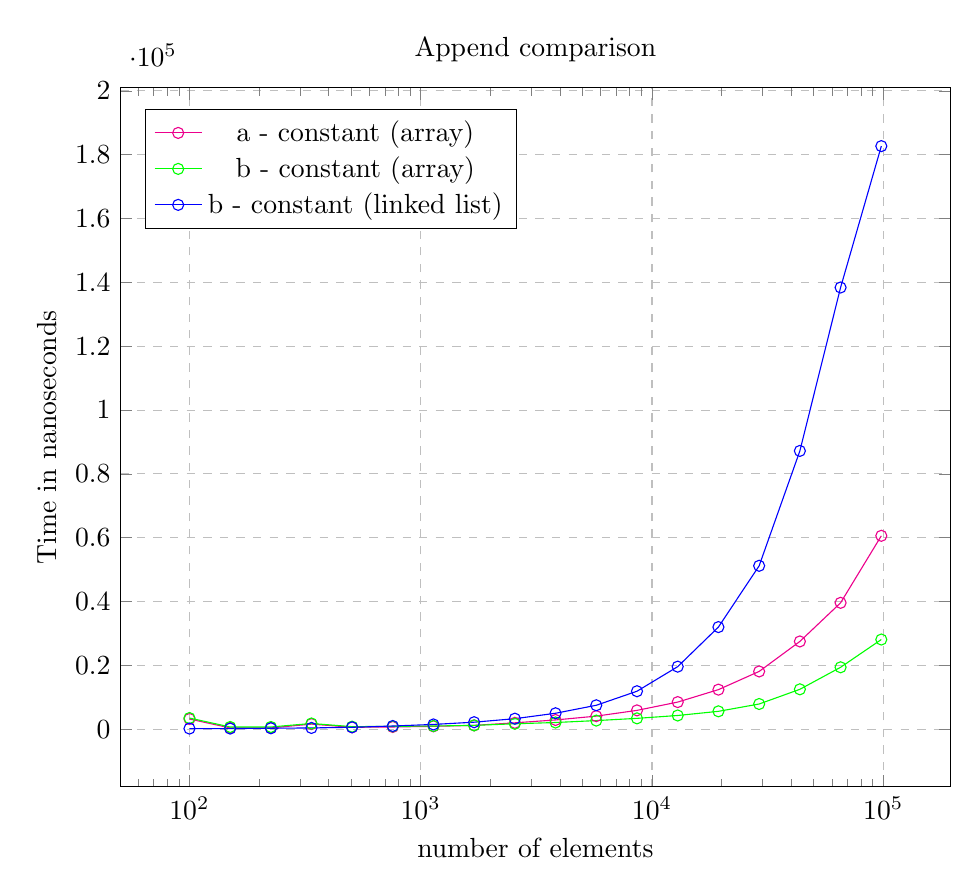
\begin{tikzpicture}
        \begin{axis}[
            title={Append comparison},
            width=\linewidth,
            xlabel={number of elements},
            ylabel={Time in nanoseconds},
            xmode=log,
            ymajorgrids=true,
            xmajorgrids=true,
            grid style=dashed,
            legend pos=north west,
        ]
        
        \addplot[
            color=magenta,
            mark=o,
            ]
            coordinates {
            (100,3200)(150,400)(225,400)(337,1600)(505,600)(757,700)(1135,900)(1702,1200)(2553,2000)(3829,2900)(5743,4100)(8614,5900)(12921,8500)(19381,12400)(29071,18100)(43606,27500)(65409,39600)(98113,60600)
            };
            \addlegendentry{a - constant (array)}

        \addplot[
            color=green,
            mark=o,
            ]
            coordinates {
            (100,3500)(150,700)(225,700)(337,1800)(505,800)(757,900)(1135,1000)(1702,1200)(2553,1700)(3829,2100)(5743,2700)(8614,3400)(12921,4300)(19381,5600)(29071,7900)(43606,12500)(65409,19400)(98113,28100)
            };
            \addlegendentry{b - constant (array)}

        \addplot[
            color=blue,
            mark=o,
            ]
            coordinates {
            (100,199)(150,199)(225,299)(337,399)(505,600)(757,1000)(1135,1499)(1702,2199)(2553,3299)(3829,4999)(5743,7500)(8614,11900)(12921,19600)(19381,32000)(29071,51201)(43606,87200)(65409,138401)(98113,182700)
            };
            \addlegendentry{b - constant (linked list)}
            
        \end{axis}
        \end{tikzpicture}
    \caption{Linked list append operation benchmark}
    \label{fig:plot1}
\end{figure}

Regarding the comparison of the three cases, I am not completely certain why they relate as they do. We might expect the linked list function to outperform the other two. And think both the array appends would yield closer results to each other, not to diverge as much as they do. I discuss more on the topic in the final \hyperref[sec:conc]{conclusion section} of this report.

\section*{Linked List Stack}

In assignment 2 I presented a way to make a dynamic stack using an array, where, whenever there was no longer any space to add new elements, I would increase the size of the stack by moving all current elements to a larger-sized array. That worked fine, but was definitely not the most optimal way to implement a stack for certain use cases. Now using the linked list structure presented here we can do a different dynamic stack implementation. This time there will not be any need to keep track if there is or not any space in the structure, since adding elements to the list involves only keeping track of the right references. 

The two functions each stack is required to have are written as so:

\begin{minted}[
frame=single,
framesep=2mm,
baselinestretch=1.2,
fontsize=\footnotesize,
]{java}
    (...)
    void push(int item) {
        add(item);
    }

    Cell pop() {
        Cell temp = first;
        remove(first.head);
        return temp;
    }
    (...)
\end{minted}

Borderline wrapper functions, but they do allow us to declare the {\tt LinkedList} class as extending the abstract class {\tt Stack} from assignment 2 and use our new code interchangeably with the previous program.
\\

\section*{Conclusion}
\label{sec:conc}
Now as stated before the linked list stack is better only for certain use cases - it is not always the better option. If we have some notion that the dynamic stack will have a certain amount of elements most often and only on some special occasions will grow larger then the array stack could prove to be better since with an array all elements are saved in memory close by. This means that working with it would yield way less cache misses and make working with the data more convenient. On the other hand if we know our data size will be growing and shrinking constantly and unpredictably, the linked list stack might be the way to go. The negative is exactly that with lists each element is not necessarily placed in memory near the previous or next, and so would require more clock cycles to be returned.

\end{document}